%harihiom
\documentclass{book}

\usepackage[english]{babel}
%\usepackage[utf8]{inputenc}
%\usepackage{amsmath}
\usepackage{tcolorbox}
\usepackage{graphicx,wrapfig,lipsum}
\usepackage{comment}
\usepackage{float}
%\usepackage{wrapfig}
%\usepackage{titlepic}
%\usepackage[colorinlistoftodos]{todonotes}
\usepackage{graphicx,epstopdf}
\usepackage{amsmath,amssymb,amsfonts,subfigure}
\usepackage{comment}
\usepackage{algorithm}
\usepackage{algpseudocode}
\usepackage{pifont}
\usepackage[normalem]{ulem}
\usepackage[english]{babel}
\usepackage[utf8x]{inputenc}
\usepackage{graphicx}
\usepackage{calc}
\usepackage{graphicx}
\usepackage{subfigure}
\usepackage{gensymb}
\usepackage{url}
\usepackage[utf8x]{inputenc}
\usepackage{amsmath}
\usepackage{graphicx}
\graphicspath{{images/}}
\usepackage{parskip}
\usepackage{fancyhdr}
\usepackage{vmargin}
\usepackage{algorithm}
\linespread{1}
\usepackage{color}
\usepackage{cite}
\usepackage{amsmath,amssymb}
\newtheorem{claim1}{Claim}
\usepackage{algpseudocode}% http://ctan.org/pkg/algorithmicx
\usepackage[compatibility=false]{caption}% http://ctan.org/pkg/caption
\setmarginsrb{3 cm}{2.5 cm}{3 cm}{2.5 cm}{1 cm}{1.5 cm}{1 cm}{1.5 cm}

%\newtheorem{theorem}{Theorem}
%\newtheorem{lemma}{Lemma}
\setcounter{chapter}{2}
\title{Probability Ideas in Computing}

\begin{document}
%\maketitle
\chapter{The Dating Problem : Decision Making under Uncertainty}

In this chapter, we will discuss an important and interesting problem related to decision making under uncertainty. In such problems, one has to make decisions in the presence of incomplete information, which makes it difficult to predict the outcome of the choosen action. 

\section{Problem Statement}

Imagine Aadhya is searching for a match for her marriage. There is a seqence of $n$ boys, $\{B_1,\ B_2,\ ..., \ B_{n}\} $, to be interviewed by her. However, she can interview only one boy at a time starting from $B_1$ to $B_n$. After every interview, she has to take one of the following two actions. 
\begin{itemize}
\item Reject the boy and move on. Once a boy is rejected, he can not be tied a knot to, in future.  
\item Accept the boy and tie a knot. Once a boy is accepted, the process ends.
\end{itemize}
In case Aadhya rejects all the boys from $B_1$ to $B_{n-1}$, she has no option but to tie a knot with $B_n$. Our aim is to devise an algorithm for Aadhya in order to maximise her probability of getting the best boy for her marriage. 

\section{Solution}
We know that it is very difficult, rather impossible, to get the best boy in this setting. The only plausible solution is to interview some boys. That will give Aadhya an idea of the fitness of the crowd. This idea can then help Aadhya in choosing the best boy. Hence, we adopt the following solution.

\begin{tcolorbox}
Aadhya interviews the first $k$ boys, $\{B_1, B_2, ..., B_k\}$. Let $B_k$ be the best match amongst these $k$ boys. Aadhya rejects all these $k$ boys mentally keeping a note of fitness of $B_k$. She continues the interviewing process and settles down as soon as she finds a match better than $B_k$. This has been illustrated in Figure \ref{boy}. The pseudocode for this solution is given in Algorithm \ref{dating}.
\end{tcolorbox}

\begin{figure}[h!]
\centering
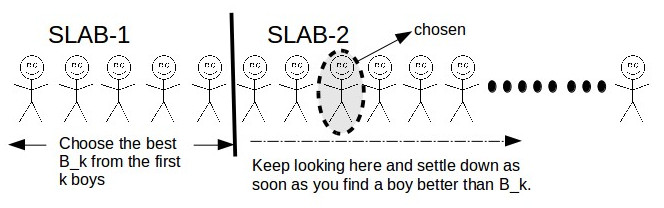
\includegraphics[width=0.9\textwidth]{boys.jpg}
\caption{Solution to the problem}
\label{boy}
\end{figure}

\begin{algorithm}[h!]
\caption{The Dating Algorithm}\label{dating}
\begin{algorithmic}[1]
\Procedure{Dating}{}
\State \textbf{Input}:- Array of the quality of $n$ boys $A[1,2,.....,n]$, $A[i]$ represents the quality of the $i_{th}$ boy, $k$
\State \textbf{Output}: $A[Best]$- The quality of the solution, $Best$- The index of the selected boy.
\State $Best\ = 0$
\For {$i\ =\ 1\ to\ k$}
\If {$A[Best] < A[i]$}
\State $Best \gets i $
\EndIf
\EndFor
\For {$i = k+1\ to\ n$}
\If {$A[Best] < A[i]$}
\State $Best \gets i$
\State break
\EndIf
\EndFor
\State return $Best$, $A[Best]$
\EndProcedure
\end{algorithmic}
\end{algorithm}



The intelligent reader might be contemplating over the optimal value of $k$. A very small value of $k$ results in a bad match since Aadhya can not see enough number of boys. This leads to her not getting the perfect picture of the fitness of the crowd. On the other hand, if $k$ is very large, there will not be enough boys left in slab-2 (refer Figure \ref{boy}) to find a good boy. Let us refer $k$ as sample size henceforth. 

\subsection{Optimal sample size}
Let $f(k)$ denote the quality of the solution when the sample size is $k$. $f(k)$ ranges from $1$ to $1000$ where the value $1000$ corresponds to the best quality and $1$ is for the worst. Our discussion above concluded that a very small as well as a very large value of $k$ results in a lesser $f(k)$. Our aim is to find the optimal value of $k$. Figure \ref{dating_k} shows a curve plotting $k$ on the X axis and $f(k)$ on the Y axis for a random sequence of $1000$ boys. It can be seen that the best choice is met for a much lesser value of $k$. 
\begin{figure}[h!]
\centering
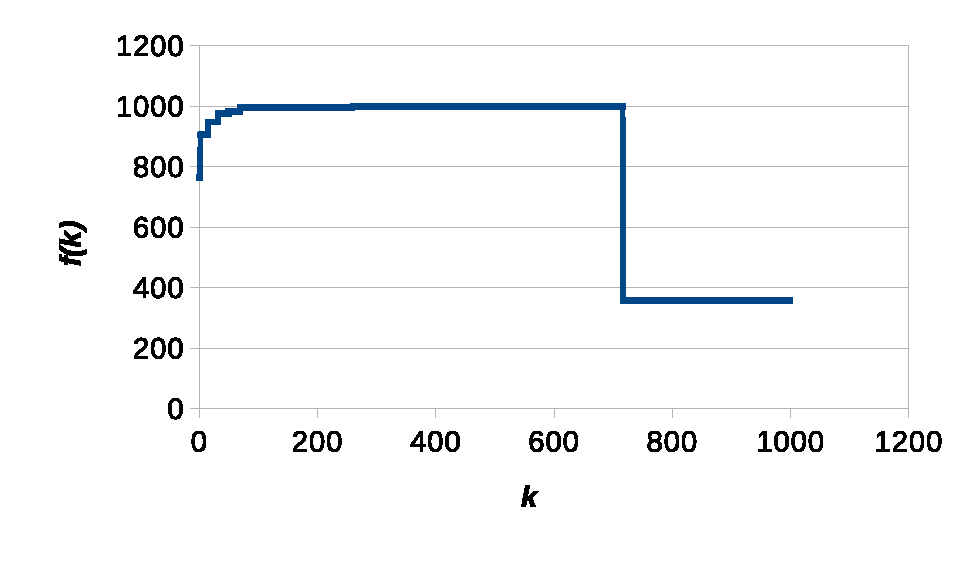
\includegraphics[scale=0.8]{dating.eps}
\caption{Plotting $k$ vs. $f(k)$}
\label{dating_k}
\end{figure} 
We will now mathematically analyse the solution and obtain a mathematical formula for the best value of $k$.

\subsection{Mathematical Analysis}

The algorithm fails to fetch the best result in one of the following two conditions.
\begin{itemize}
\item \textbf{When the best boy falls in the first slab (Firstly interviewed $k$ boys(Our sample of the crowd))}. 
\item \textbf{When the best boy falls in the second slab but his position is after at least one boy who is better than $B_k$} (best boy chosen from the sample). This is shown in Figure \ref{hero}. Here, we end up picking a suboptimal solution which is sandwiched between the boy at the $k+1_{th}$ location boy and the best boy. 
\end{itemize}

\begin{figure}[h]
\centering
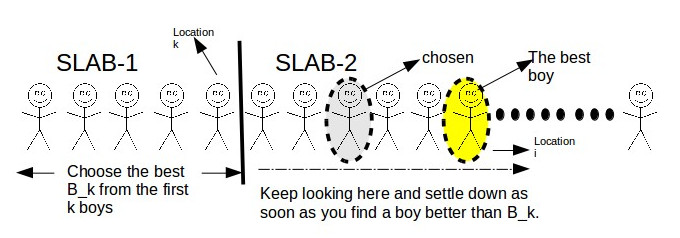
\includegraphics[width=0.9\textwidth]{hero.jpg}
\caption{Choosing someone who is not the best}
\label{hero}
\end{figure}

$Pr$(Best boy is in the first $k$ locations) = $ \frac{k}{n}$, since there are $k$ ways in which the best boy can be present at any of the first $k$ locations and the total number of locations to be present at are $n$. \\

A boy is said to be pseudo-best if his quality is greater than $B_k$ and lesser than the quality of the best boy.
 
Now, for the algorithm to fetch the best boy, both of the following conditions should hold.
\begin{enumerate}
\item The best boy should be present after the first $k$ locations (in the second slab). 
\item If the location of the best boy is $i$, the the quality of all the boys in locations $[k+1,i-1]$ should be lesser than the quality of $B_k$. In other words no pseudo-best boy should be present in the locations $[k+1,i-1]$.
\end{enumerate}

Hence, $Pr$(We get the best boy)= $Pr$(Best boy is at the location $i$ and no pseudo-best boy is present in the locations $[k+1,i-1]$ ).\\

\begin{equation}\label{eq1}
\text{Given a location $i$, $Pr$(Best boy is present at this location) = $1/n$.}
\end{equation}

Let us divide the queue of boys in three slabs as shown in Figure \ref{slabs}.

\begin{figure}[h!]
\centering
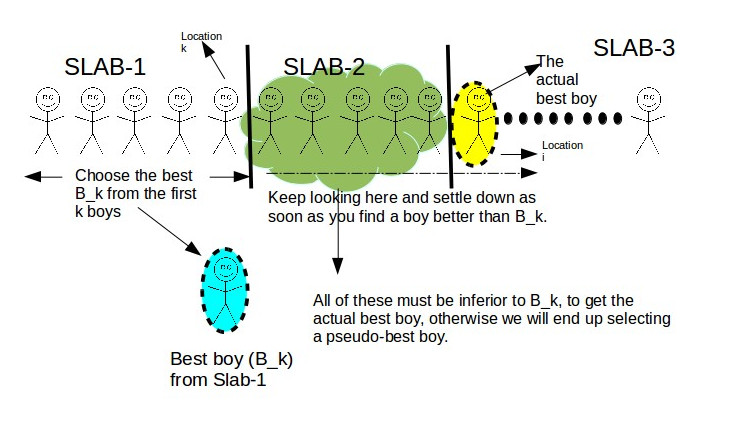
\includegraphics[width=0.9\textwidth]{slabs.jpg}
\caption{Choosing the best}
\label{slabs}
\end{figure}

\begin{center}
$Pr$(The best boy from locations $1$ to $i-1$ is present before the location $k+1$)= $\frac{k}{i-1}$
\end{center}


\begin{equation}\label{eq2}
\text{Hence, $Pr$(Pseudo-best boy is not there at locations $[k+1,i-1]$) = $\frac{k}{i-1}$..}
\end{equation}



From equations \ref{eq1} and \ref{eq2} \\
\begin{center}
$Pr$(winning when the best boy is at the location $i$) = $\frac{1}{n} \times \frac{k}{i-1}$\\
\end{center}

Now the location of the best boy can vary from $k+1$ to $n$. Taking all these cases in account,\\

$Pr$(We end up choosing the best boy)= $\sum_{i=k+1}^n \frac{1}{n} \times \frac{k}{i-1}$\\

= $\frac{k}{n} \sum_{i=k+1}^n \frac{1}{i-1}$\\

= $\frac{k}{n} \sum_{i=k}^{n-1} \frac{1}{i}$\\

= $\frac{k}{n} \int_{k}^{n} \frac{1}{i} di$ (we replaced $n-1$ by $n$ assuming $n$ is a very large number)\\

= $\frac{k}{n}|log\ i|_{k}^{n}$\\

=$\frac{k}{n} (log\ n - log\ k)$\\

\[
 \boxed{f(k)\ =\ \frac{k}{n} (log\ n - log\ k)}
 \]
 
 We want to find a $k$ which maximises this probability. Hence, we differentiate the above equation.
 
 $f'(k)=\ \frac{1}{n} (log\ n\ -\ log\ k) + \frac{k}{n} \times \frac{-1}{k}$\\
 
 Equating to $0$,
 
 $\frac{1}{n} (log\ n\ -\ log\ k) + \frac{k}{n} \times \frac{-1}{k}\ =0$\\
 
 $ (log\ n\ -\ log\ k\ -\ 1\ = 0)$\\
 
 or, $log\ n\ -\ log_e\ e\ =\ log\ k$\\
 
 or, $log\ \frac{n}{e}\ =\ log\ k$\\
 
 or, 
\[
 \boxed{k=\ \frac{n}{e}}
 \]



\bibliographystyle{plain}
\bibliography{book}

\end{document}





